\chapter{人形机器人全身动作重定向}%20页


\section{引言}
人机交互(Human–Robot Interaction,HRI)是仿人机器人研究中的重要方向,而运动模仿则是实现自然、高效交互行为的核心手段之一。由于人体与机器人在运动学结构、关节自由度配置以及运动范围等方面存在显著差异,如何将人体动作合理映射到机器人平台上,仍然是运动模仿与动作重定向中的关键挑战。

现有的动作重定向方法通常可分为基于关节空间和基于笛卡尔空间的两类。前者侧重于保持人体与机器人在关节构型层面的相似性,但往往难以保证末端执行器在任务空间中的精确运动;后者则以末端轨迹跟踪为主要目标,但容易忽略整体肢体构型的一致性,从而导致机器人运动不自然。这种构型一致性与任务空间精度之间的权衡,限制了重定向结果在复杂交互场景中的适用性。

针对上述问题,本章在已有动作重定向研究的基础上,对传统重定向框架进行了改进,通过在关节空间构型约束与笛卡尔空间末端跟踪之间建立协调机制,实现了对人体上肢动作的有效映射。在保证机器人手臂整体构型与人体动作保持一致的同时,该方法能够显著提升末端执行器位置与姿态的跟踪精度,从而兼顾运动自然性与任务可执行性。实验结果表明,该重定向方法在不同动作类型与操作场景下均表现出良好的稳定性与适应性,为后续结合学习方法进行全身动作生成与控制奠定了基础。

近年来,利用人体运动数据对机器人进行示教与运动生成,已成为简化机器人运动编程与学习过程的一种重要途径 \cite{fu2024mobile, he2024learning, butepage2020imitating, kulic2016anthropomorphic}。通过观测和映射人类动作,机器人能够在无需显式建模复杂任务逻辑的情况下获得具有较强表现力和适应性的运动行为,这对于提升仿人机器人的自然性、自主性以及人机交互能力具有重要意义 \cite{chi2024universal, bahl2022human}。尽管该方向已取得一定进展 \cite{ishiguro2020bilateral, ramos2018humanoid},但在结构受限的真实机器人平台上实现稳定且精确的人体运动模仿,仍然面临诸多挑战 \cite{kim2009stable}。

从运动映射的角度来看,人体到机器人的动作模仿通常可抽象为一个\emph{动作重定向(motion retargeting)}问题,即在满足机器人自身运动学与动力学约束的前提下,将人体动作合理映射到机器人关节空间或任务空间中。由于人体与机器人在自由度数量、关节拓扑结构、运动范围以及力矩能力等方面存在显著差异,人体动作往往无法被机器人直接复现,这使得动作重定向成为运动模仿中的核心问题之一。

现有的动作重定向方法大致可以分为基于学习的方法和基于模型的方法。在动画与虚拟角色控制领域,强化学习被广泛用于从人体动作数据中学习复杂运动策略,并在多种任务中展现出良好的泛化能力与风格一致性 \cite{peng2018deepmimic, peng2021amp, won2020scalable, luo2023perpetual}。然而,将此类方法直接应用于真实仿人机器人仍然面临仿真到现实差距(sim-to-real gap)的问题,尤其是在关节力矩限制、硬件安全性以及高精度末端控制等方面存在明显挑战 \cite{bohez2022imitate, tang2024humanmimic}。

相比之下,基于模型的动作重定向方法由于其可解释性强、对物理约束处理明确,在真实机器人系统中仍被广泛采用。根据映射空间的不同,这类方法通常可进一步分为基于笛卡尔空间和基于关节空间的重定向策略。基于笛卡尔空间的方法通常以末端执行器位姿跟踪为主要目标,通过逆运动学或优化方法实现任务空间误差最小化 \cite{koenemann2014real, arduengo2021human}。这类方法在任务执行精度方面具有优势,但由于缺乏对整体肢体构型的约束,容易导致机器人运动不自然,且在存在避障或关节限制时可行性较差。相对而言,基于关节空间的方法更关注机器人与人体在构型层面的相似性,能够生成较为自然的运动,但往往难以保证末端执行器在任务空间中的精确跟踪,从而限制了其在精细操作任务中的应用。

因此,\textbf{如何在动作重定向过程中同时兼顾关节构型一致性与末端执行器的任务空间精度},成为当前类人机器人运动模仿研究中的一个关键问题。现有方法通常在这两者之间进行权衡,尚难以在统一框架下有效协调二者。

基于上述背景,本章在已有动作重定向研究的基础上,对传统的重定向流程进行了系统梳理与分析,并引入一种结合关节空间构型约束与笛卡尔空间任务优化的重定向建模思路。该思路以人体手臂运动为示教源,通过建立人体与机器人之间的几何对应关系,
在满足机器人关节空间约束的前提下,引入基于笛卡尔空间的优化机制,对末端执行器运动进行精确调节,从而在构型一致性与任务精度之间取得更为平衡的解。

需要强调的是,本章关注的重点在于\emph{动作重定向问题本身的建模方式与约束处理机制},其目的在于为后续章节中基于学习的全身动作生成与控制策略提供稳定、合理的低层动作映射基础。

\section{预备知识}

为后续人形机器人全身动作重定向与任务优先级控制模型的构建,本节对空间位姿描述与坐标变换方法,以及二次规划优化的基本理论进行简要回顾。这些内容构成后续全身运动学建模与优化求解的理论基础。



\subsection{空间位姿描述与坐标变换基础}

在人形机器人运动控制问题中,空间中任一点或刚体的状态通常由位置与姿态两部分组成。为统一描述空间几何关系,首先定义参考坐标系。设 $\{A\}$ 为参考坐标系,则空间点 $P$ 在坐标系 $\{A\}$ 下的位置向量表示为

\begin{equation}
	{}^{A}\mathbf{p} =
	\begin{bmatrix}
		p_x \\
		p_y \\
		p_z
	\end{bmatrix}.
\end{equation}

其中,上标 $A$ 表示该向量在坐标系 $\{A\}$ 下表达。图~\ref{fig:frameA} 给出了三维直角坐标系 $\{A\}$ 的示意图。

\begin{figure}[htbp]
	\centering
	\includegraphics[width=0.45\linewidth]{Figure/chapter2/frame_A.png}
	\caption{三维直角坐标系 $\{A\}$ 示意图}
	\label{fig:frameA}
\end{figure}

刚体姿态可通过附着于刚体的坐标系 $\{B\}$ 相对于参考系 $\{A\}$ 的关系描述。设 
$\{\hat{\mathbf{x}}_B,\hat{\mathbf{y}}_B,\hat{\mathbf{z}}_B\}$ 
为 $\{B\}$ 的三个单位基向量,则其在 $\{A\}$ 中的表达可构成旋转矩阵

\begin{equation}
	{}^{A}_{B}\mathbf{R} =
	\begin{bmatrix}
		{}^{A}\hat{\mathbf{x}}_B &
		{}^{A}\hat{\mathbf{y}}_B &
		{}^{A}\hat{\mathbf{z}}_B
	\end{bmatrix}.
\end{equation}

该旋转矩阵满足正交性条件

\begin{equation}
	{}^{A}_{B}\mathbf{R}^{T} \, {}^{A}_{B}\mathbf{R} = \mathbf{I}_3,
	\qquad
	{}^{A}_{B}\mathbf{R}^{-1} = {}^{B}_{A}\mathbf{R}.
\end{equation}

图~\ref{fig:frameAB} 给出了两个坐标系 $\{A\}$ 与 $\{B\}$ 的空间关系示意图。

\begin{figure}[htbp]
	\centering
	\includegraphics[width=0.75\linewidth]{Figure/chapter2/frame_A_B.png}
	\caption{坐标系 $\{A\}$ 与 $\{B\}$ 的空间关系示意图}
	\label{fig:frameAB}
\end{figure}

若两个坐标系原点重合,仅存在旋转关系,则任意向量在两个坐标系中的表达满足
${}^{A}\mathbf{p} = {}^{A}_{B}\mathbf{R}\,{}^{B}\mathbf{p}$。若两坐标系姿态相同,仅存在平移关系,则有
${}^{A}\mathbf{p} = {}^{B}\mathbf{p} + {}^{A}\mathbf{p}_{B\mathrm{ORG}}$。其中 ${}^{A}\mathbf{p}_{B\mathrm{ORG}}$ 表示坐标系 $\{B\}$ 原点在 $\{A\}$ 下的位置。

综合平移与旋转,可构造齐次变换矩阵

\begin{equation}
	{}^{A}_{B}\mathbf{T} =
	\begin{bmatrix}
		{}^{A}_{B}\mathbf{R} & {}^{A}\mathbf{p}_{B\mathrm{ORG}} \\
		\mathbf{0}_{1\times 3} & 1
	\end{bmatrix}
	\in SE(3),
\end{equation}

则空间点在不同坐标系之间的映射关系可统一表示为

\begin{equation}
	\begin{bmatrix}
		{}^{A}\mathbf{p} \\
		1
	\end{bmatrix}
	=
	{}^{A}_{B}\mathbf{T}
	\begin{bmatrix}
		{}^{B}\mathbf{p} \\
		1
	\end{bmatrix}.
\end{equation}

上述空间位姿表示与坐标变换关系构成了人形机器人几何建模的基础框架,为后续全身运动学推导以及人体动作到机器人结构之间的重定向映射提供了统一的数学描述形式。



\subsection{二次规划与约束优化基础}
二次规划(Quadratic Programming, QP)的一般形式为
\begin{equation}
	\begin{aligned}
		\min_{\mathbf{x}} \quad &
		\frac{1}{2}\mathbf{x}^T \mathbf{G}\mathbf{x}
		+
		\mathbf{h}^T \mathbf{x} \\
		\text{s.t.} \quad &
		\mathbf{A}\mathbf{x} = \mathbf{b}, \\
		&
		\mathbf{C}\mathbf{x} \le \mathbf{d},
	\end{aligned}
	\label{eq:qp_general}
\end{equation}
其中 $\mathbf{G} \succeq 0$ 为半正定矩阵,$\mathbf{A}\mathbf{x} = \mathbf{b}$ 和 $\mathbf{C}\mathbf{x} \le \mathbf{d}$ 分别表示等式与不等式约束。

当仅存在等式约束时,可构造 Lagrange 函数
\begin{equation}
	\mathcal{L}(\mathbf{x},\boldsymbol{\lambda})
	=
	\frac{1}{2}\mathbf{x}^T \mathbf{G}\mathbf{x}
	+
	\mathbf{h}^T \mathbf{x}
	+
	\boldsymbol{\lambda}^T(\mathbf{A}\mathbf{x}-\mathbf{b}),
\end{equation}
对 $\mathbf{x}$ 与 $\boldsymbol{\lambda}$ 求偏导并令其为零,可得到一阶最优性条件,整理后得到 KKT 方程组
\begin{equation}
	\begin{bmatrix}
		\mathbf{G} & \mathbf{A}^T \\
		\mathbf{A} & \mathbf{0}
	\end{bmatrix}
	\begin{bmatrix}
		\mathbf{x} \\
		\boldsymbol{\lambda}
	\end{bmatrix}
	=
	\begin{bmatrix}
		-\mathbf{h} \\
		\mathbf{b}
	\end{bmatrix},
\end{equation}
通过求解该线性方程组即可获得二次规划问题的最优解。

另一方面,在人形机器人运动学中,设广义关节变量为 $\mathbf{q} \in \mathbb{R}^n$,任务空间变量记为 $\mathbf{x}$,则末端或任务点的位姿满足
\begin{equation}
	\mathbf{x} = f(\mathbf{q}),
\end{equation}
其微分形式为
\begin{equation}
	\dot{\mathbf{x}} = \mathbf{J}(\mathbf{q}) \dot{\mathbf{q}},
	\label{eq:task_velocity_mapping}
\end{equation}
其中 $\mathbf{J}(\mathbf{q})$ 为雅可比矩阵。

给定期望的任务空间速度 $\dot{\mathbf{x}}_d$,可以构造任务空间速度误差
\begin{equation}
	\mathbf{e}_v = \mathbf{J}(\mathbf{q}) \dot{\mathbf{q}} - \dot{\mathbf{x}}_d,
\end{equation}
并以其加权二范数作为代价函数
\begin{equation}
	\min_{\dot{\mathbf{q}}} \;
	\frac{1}{2} \mathbf{e}_v^T \mathbf{W} \mathbf{e}_v
	=
	\frac{1}{2}
	\big(
	\mathbf{J}(\mathbf{q}) \dot{\mathbf{q}} - \dot{\mathbf{x}}_d
	\big)^T
	\mathbf{W}
	\big(
	\mathbf{J}(\mathbf{q}) \dot{\mathbf{q}} - \dot{\mathbf{x}}_d
	\big),
	\label{eq:quadratic_cost_from_jacobian}
\end{equation}
其中 $\mathbf{W} \succeq 0$ 为任务空间加权矩阵。展开式\eqref{eq:quadratic_cost_from_jacobian} 可得
\begin{equation}
	\frac{1}{2} \dot{\mathbf{q}}^T \big( \mathbf{J}^T \mathbf{W} \mathbf{J} \big) \dot{\mathbf{q}}
	-
	\big( \mathbf{J}^T \mathbf{W} \dot{\mathbf{x}}_d \big)^T \dot{\mathbf{q}}
	+
	\text{const},
\end{equation}
从而可以识别出
\begin{equation}
	\mathbf{x} \equiv \dot{\mathbf{q}}, \quad
	\mathbf{G} = \mathbf{J}^T \mathbf{W} \mathbf{J}, \quad
	\mathbf{h} = - \mathbf{J}^T \mathbf{W} \dot{\mathbf{x}}_d,
\end{equation}

即由机器人雅可比映射自然得到二次规划中的二次型代价形式。进一步结合关节速度限制、末端约束等线性约束,即可将全身运动学问题统一表示为式\eqref{eq:qp_general} 所示的标准 QP 形式,为后续的人形机器人动作重定向提供统一的优化求解框架。




\section{方法}
\subsection{动作模仿系统设计}
图~\ref{fig:System_Block_Diagram} 展示了本文所构建的全身动作模仿系统整体框架。系统主要由视觉采集系统、上位处理器、下位处理器以及机械运动系统四个部分组成,各模块协同工作以实现人形机器人全身动作模仿。

\begin{figure}[htbp]
	\centering
	\includegraphics[width=0.9\linewidth]{Figure/chapter2/system_frame.png}
	\caption{全身动作模仿系统整体框架}
	\label{fig:System_Block_Diagram}
\end{figure}

视觉采集系统采用标准的 RGB-D 摄像设备,本文实验中使用 Intel RealSense D435 深度相机。摄像头安装于被试者正前方,距地面约 1.5 m,用于实时获取人体运动图像及对应的深度信息。采集到的数据通过 USB 接口传输至上位处理器进行处理。

上位处理器为一台 PC,负责完成人体姿态信息的提取与预处理。具体而言,上位处理器对输入的 RGB 图像进行人体姿态估计,提取人体全身关键点的二维信息,并进一步结合深度数据恢复三维关键点位置。为降低传感噪声对后续动作重定向的影响,本文对三维关键点序列引入卡尔曼滤波进行平滑处理。处理后的关键点数据通过 ROS 通信机制发送至下位处理器。

为清晰描述人体与机器人之间的映射关系,
图~\ref{fig:human_robot_compare} 给出了人体关键点结构与机器人本体结构的对比示意图。
图~\ref{fig:human_keypoints_sub} 为人体关键点定义,
图~\ref{fig:robot_structure_sub} 为机器人本体结构及关节坐标系定义。

\begin{figure}[htbp]
	\centering
	\begin{subfigure}[b]{0.32\textwidth}
		\centering
		\includegraphics[width=\linewidth]{Figure/chapter2/human_body.png}
		\caption{人体关键点定义}
		\label{fig:human_keypoints_sub}
	\end{subfigure}
	\hfill
	\begin{subfigure}[b]{0.52\textwidth}
		\centering
		\includegraphics[width=\linewidth]{Figure/chapter2/M04_body.png}
		\caption{人形机器人本体结构与关节旋转}
		\label{fig:robot_structure_sub}
	\end{subfigure}
	\caption{人体关键点与机器人本体结构对比示意图}
	\label{fig:human_robot_compare}
\end{figure}

人体侧关键点包括肩关节($S$)、肘关节($E$)、腕关节($W$)、髋关节($H$)、膝关节($K$)、踝关节($A$)以及躯干参考点($P$、$O$)等。通过人体姿态估计算法可获取上述关键点在相机坐标系下的三维空间位置坐标,从而构建人体全身骨架的几何拓扑结构。机器人侧则建立与人体结构相对应的串联关节连杆模型,并在各关节处定义局部连杆坐标系 $\{X,Y,Z\}$。各关节旋转采用右手坐标系约定,并按照 Roll–Pitch–Yaw 顺序定义转动自由度。该统一的坐标描述方式为人体—机器人之间的几何映射与运动学重定向提供了理论基础。

下位处理器用于执行动作重定向计算与机器人控制指令生成。在接收到人体三维关键点数据后,系统首先基于人体几何模型计算对应的人体关节角度,该关节角度作为机器人动作重定向问题的初始参考。随后,通过迭代优化求解满足机器人关节物理约束并同时逼近人体末端运动目标的关节角解。最终得到的目标关节角通过 CAN 总线发送至机械运动系统,用于驱动机器人执行相应的全身动作。

机械运动系统由机器人双臂、双腿、电机及其驱动模块构成。本文所使用的仿人机器人平台为自主研发系统。上肢每条机械臂具有六个自由度,包括肩关节三自由度(屈伸、外展内收、旋内外)、肘关节屈伸、前臂旋前旋后以及腕关节屈伸;下肢包括髋关节三自由度、膝关节屈伸以及踝关节俯仰。该结构能够满足机器人在三维空间内完成复杂全身动作的运动学需求,为人体动作的有效重定向提供了硬件基础。


\section{改进重定向}
\subsection{人体肩关节几何建模}
由于肩关节和肘关节主要影响手臂的运动,而手腕主要影响手的运动,本研究重点对肩关节和肘关节进行几何建模。为清楚说明肩关节和肘关节的建模方法,下面以左臂的建模过程进行说明。

如图 \ref{fig:Modeling_of_shoulder} 所示,点 $S$ 表示左臂的肩关节,点 $E$ 表示左臂的肘关节,点 $M$ 则位于 Y 轴上,距离为 $a$ 的一点。
\begin{figure}[h]
	\centering
	\includegraphics[width=0.4\textwidth]{Figure/chapter2/Fig3.png}
	\caption{左手肩关节建模。}
	\label{fig:Modeling_of_shoulder}
\end{figure}


根据上述定义,可以证明 $|\bm{SM}| = a$。通过姿态估计,可以获得各关键点在相机坐标系下的坐标,分别为 $S(x_0, y_0, z_0)$、$E(x_1, y_1, z_1)$ 以及 $M(x_0, y_0 - a, z_0)$。以点 $S$ 为原点建立肩关节局部坐标系后,各点在该坐标系下的坐标可表示为 $S(0, 0, 0)$、$E(x_1 - x_0,\, y_1 - y_0,\, z_1 - z_0)$ 以及 $M(0,\, -a,\, 0)$。

点 $E$ 在平面 $(ZSM)$ 上的正交投影记为点 $F$,其坐标为 $F(0,\, y_0 - y_1,\, z_1 - z_0)$。向量 $\bm{SE}$ 在平面 $(ZSM)$ 上的投影与 $Y$ 轴负方向之间的夹角定义为 $\theta_1$,即 $\angle FSM = \theta_1$,其中 $\theta_1$ 表示肩关节的屈伸角;向量 $\bm{SE}$ 与其在平面 $(ZSM)$ 上投影之间的夹角定义为 $\theta_2$,即 $\angle FSE = \theta_2$,其中 $\theta_2$ 表示肩关节的外展–内收角。

在上述几何关系下,可在三角形 $\triangle FSM$ 中求解角度 $\theta_1$,根据余弦定理有
\begin{equation}
\theta_{1}
= \arccos\!\left(
\frac{|\bm{SF}|^{2} + |\bm{SM}|^{2} - |\bm{FM}|^{2}}
{2\,|\bm{SF}|\,|\bm{SM}|}
\right)
= \arccos\!\left(
\frac{y_0 - y_1}{|\bm{SF}|}
\right),
\label{eq:theta1}
\end{equation}

其中角度 $\theta_1$ 的符号可由 $z_1 - z_0$ 的符号确定:当 $z_1 - z_0 > 0$ 时,表示手臂向前摆动;当 $z_1 - z_0 < 0$ 时,表示手臂向后摆动。同理,在三角形 $\triangle FSE$ 中可求解肩关节外展–内收角 $\theta_2$,其表达式为

\begin{equation}
\theta_{2}
= \arccos\!\left(
\frac{|\bm{SF}|^{2} + |\bm{SE}|^{2} - |\bm{FE}|^{2}}
{2\,|\bm{SF}|\,|\bm{SE}|}
\right).
\label{eq:theta2}
\end{equation}



\subsection{人体肘关节几何建模}
如图~\ref{fig:Modeling of elbow}(\textbf{a}) 所示,$W$ 表示手腕的实际位置,$W'$ 表示手腕的假定初始位置(此时 $\theta_{3} = 0$)。角度 $\theta_{3}$ 定义为从肘部指向手腕的向量 $\bm{EW}$ 与其初始位置向量 $\bm{EW'}$ 之间的夹角;角度 $\theta_{4}$ 定义为向量 $\bm{EW}$ 与向量 $\bm{SE}$ 的延长线之间的夹角。


\begin{figure}[H]
	\centering
	%\isPreprints{}{% This command is only used for ``preprints''.
		\begin{adjustwidth}{0cm}{0cm}
			\subfloat[\centering]{\includegraphics[width=7.5cm]{Figure/chapter2/Fig4.png}}
			\label{fig:arm joint angles are non zero}
			\hfill
			\subfloat[\centering]{\includegraphics[width=5.4cm]{Figure/chapter2/Fig5.png}}
			\label{fig:arm joint angles are zero}
			
		\end{adjustwidth}
  \caption{肘关节建模。(\textbf{a})当手臂关节角不为零时的肘关节坐标系,其中 $\theta_{3}$ 表示肩关节外-内旋角,$\theta_{4}$ 表示肘关节屈伸角的补角。(\textbf{b})当手臂所有关节角均为零时的肘关节坐标系。}
		\label{fig:Modeling of elbow}
	\end{figure} 

当手腕位于位置 $W'$ 时,肘关节的局部坐标系记为 $E X_{1} Y_{1} Z_{1}$。假设手臂的初始状态为 $\theta_{1}$、$\theta_{2}$、$\theta_{3}$ 和 $\theta_{4}$ 均为零,则此时肘关节坐标系的定义如图~\ref{fig:Modeling of elbow}(\textbf{b}) 所示。


通过姿态估计,可以获得点 $S$、$E$ 和 $W$ 在相机坐标系下的绝对坐标,分别为 $S(x_{0}, y_{0}, z_{0})$、$E(x_{1}, y_{1}, z_{1})$ 和 $W(x_{2}, y_{2}, z_{2})$。在以肩关节为原点建立的相对坐标系下,手腕点 $W$ 的坐标可表示为 $W(x_{2}-x_{0},\, y_{2}-y_{0},\, z_{2}-z_{0})$。

如图 \ref{fig:Modeling of elbow}(\textbf{a}) 所示,在以肩关节为原点建立的相对坐标系中,肩关节外旋角 $\theta_4$ 可通过向量 $\bm{SE}$ 与向量 $\bm{EW}$ 的点积计算得到。


\begin{eqnarray}
\theta_{4} = \arccos\left[\frac{\bm{SE}\cdot\bm{EW}}{|\bm{SE}||\bm{EW}|}\right]
\end{eqnarray}

人体肘关节的活动范围为 $\pi - \theta_{4}$,其中向量 $\bm{EW}$ 的坐标为 $(x_{1} - x_{2},\, y_{1} - y_{2},\, z_{2} - z_{1})$。

为求解 $\theta_{3}$,已知实际手腕位置 $W$,首先需要计算向量 $\bm{HW}$。如图 \ref{fig:Modeling of elbow}(\textbf{a}) 所示,$Y_1$ 轴定义为始终指向肩关节到肘关节的连线,即沿向量 $\bm{SE}$ 的方向。由于 $\theta_{4}$ 已确定,无论 $\theta_{3}$ 如何变化,向量 $\bm{EW}$、$\bm{EW'}$ 与 $\bm{EH}$(即 $Y_1$ 轴)之间的夹角均保持为 $\theta_{4}$,换言之,连接肘关节与手腕的线 $\bm{EW'}$ 围绕 $Y_1$ 轴旋转形成向量 $\bm{EW}$。


\begin{gather}
|\bm{EW'}|= |\bm{EW}| \\
|\bm{EH}|= |\bm{EW'}|*cos\theta_4 \\
\bm{EH} =|\bm{EH}|\ast\frac{\bm{SE}}{|\bm{SE}|}
\end{gather}

因此,通过 $\bm{HW} = \bm{EW} - \bm{EH}$ 可以得到向量 $\bm{HW}$。需要注意的是,虽然肩关节坐标系在手臂运动过程中保持固定,但肘关节坐标系会随姿态变化而改变方向,如图 \ref{fig: Rotational schematic of the shoulder coordinate system} 所示。在手臂运动过程中,肘关节坐标系会旋转到新的状态。在图 \ref{fig: Rotational schematic of the shoulder coordinate system} 中,$Z_1$ 轴的方向会随着 $\theta_1$ 的值而变化,$Z_1'$ 轴表示 $Z_1$ 轴从肘关节平移到肩关节的位置。沿 $Z_1'$ 轴的方向向量记为 $\bm{p}$,且满足 $\bm{p} \perp \bm{m}$ 且 $|\bm{p}| = 1$,因此 $\bm{p} = (0, \sin\theta_1, -\cos\theta_1)$。如图所示,$\bm{p}$ 表示当手腕达到位置 $W'$ 时,肘关节处 $Z_1$ 轴的方向。已知向量 $\bm{HW}$ 以及与 $\bm{HW'}$ 平行的方向向量 $\bm{p}$,即可求得 $\theta_3$。


\begin{figure}[H]
\centering
%\isPreprints{}{% This command is only used for ``preprints''.
	\begin{adjustwidth}{0cm}{0cm}
		\subfloat[\centering]{\includegraphics[width=5cm]{Figure/chapter2/Fig6_a.png}}
		\label{fig: Shoulder motion as an acute angle}
		\hfill
		\subfloat[\centering]{\includegraphics[width=5cm]{Figure/chapter2/Fig6_b.png}}
		\label{fig: Shoulder motion as an obtuse angle}
		
	\end{adjustwidth}
\caption{手臂运动过程中肩关节坐标系的旋转示意图。(\textbf{a})肩关节屈伸运动为锐角示意,(\textbf{b})肩关节屈伸运动为钝角示意。}
\label{fig: Rotational schematic of the shoulder coordinate system}
\end{figure} 

\subsection{人体髋关节几何建模}

为清晰描述人体下肢关键点的空间关系,
图~\ref{fig:human_keypoints_sub}  给出了人体全身关键点定义示意图。
其中 $H$、$K$、$A$ 分别表示髋、膝和踝关节,

与上肢几何建模方法类似,
下肢髋关节角度可通过关键点之间的空间向量关系进行求解。
设姿态估计得到关键点在相机坐标系下的三维位置为
$\mathbf{p}_H,\mathbf{p}_K,\mathbf{p}_O,\mathbf{p}_P \in \mathbb{R}^3$,
则可构建如下几何关系。。

\paragraph{(1)骨盆局部坐标系构建}

如图~\ref{fig:hip_leg_geometry}(a) 所示,定义骨盆参考向量 $\mathbf{v}_{OH} = \mathbf{p}_H - \mathbf{p}_O$,
以及躯干方向向量 $\mathbf{v}_{OP} = \mathbf{p}_P - \mathbf{p}_O$。由上述两个向量可构建骨盆局部参考平面。该平面的法向量定义为
\begin{equation}
	\mathbf{n}_{HP}
	=
	\mathbf{v}_{OP} \times \mathbf{v}_{OH}.
	\label{eq:hip_normal}
\end{equation}


\begin{figure}[htbp]
	\centering
	%--------- (a) 骨盆局部坐标系 ---------
	\begin{subfigure}[c]{0.5\textwidth}
		\centering
		\begin{tikzpicture}[>=Stealth, line cap=round, line join=round, scale=1.2]
			% 全局坐标轴
			\draw[->] (0,0) -- (0,3.0) node[above] {$Z$};
			\draw[->] (0,0) -- (2.9,0) node[right] {$Y$};
			\draw[->] (0,0) -- (-2,-1) node[left] {$X$};
			
			% 关键点 O, P, H
			\coordinate (O) at (0,0);       % 骨盆中心
			\coordinate (P) at (0.9,2.1);   % 上躯干参考点
			\coordinate (H) at (2.0,-0.5);  % 髋关节中心
			
			% 骨盆平面 O-P-H
			\fill[orange!20, draw=orange!60]
			(O) -- (P) -- (H) -- cycle;
			
			% 向量 v_OP, v_OH
			\draw[thick,->] (O) -- (P)
			node[pos=0.35,right=4pt,yshift=2pt] {$\mathbf{v}_{OP}$};
			\draw[thick,->] (O) -- (H)
			node[midway,below=2pt] {$\mathbf{v}_{OH}$};
			
			% 法向量 n_HP
			\coordinate (nHP) at (0.5,2.0);
			\draw[thick,->] (O) -- (nHP)
			node[pos=1.05,left=-9pt,yshift=4pt] {$\mathbf{n}_{HP}$};
			
			% 侧向轴 r
			\coordinate (rvec) at (2.3,0.45);
			\draw[thick,->] (O) -- (rvec)
			node[below=2pt] {$\mathbf{r}$};
			
			% 标注点 O, P, H
			\fill (O) circle (1.2pt) node[below left=1pt] {$O$};
			\fill (P) circle (1.2pt) node[above right=1pt] {$P$};
			\fill (H) circle (1.2pt) node[below right=1pt] {$H$};
		\end{tikzpicture}
		\caption{骨盆局部坐标系构建}
		\label{fig:pelvis_local_frame_sub}
	\end{subfigure}
	\hfill
	%--------- (b) 髋膝几何关系 ---------
	\begin{subfigure}[c]{0.46\textwidth}
		\centering
		% 这里用你导出的那张髋膝几何图的文件名替换 leg_geometry.pdf
		\includegraphics[width=\linewidth]{Figure/chapter2/leg_geometry.png}
		\caption{髋膝关节几何关系}
		\label{fig:hip_knee_geometry_sub}
	\end{subfigure}
	
	\caption{人体下肢髋膝关节几何建模示意图}
	\label{fig:hip_leg_geometry}
\end{figure}





向量 $\mathbf{n}_{HP}$ 表示骨盆横向方向,用于刻画身体左右方向的空间参考。

为构建右手坐标系,引入侧向单位向量


\begin{equation}
	\mathbf{r}
	=
	\frac{\mathbf{v}_{OH} \times \mathbf{n}_{HP}}
	{\left\|\mathbf{v}_{OH} \times \mathbf{n}_{HP}\right\|},
	\label{eq:hip_r}
\end{equation}

至此,在髋关节处建立局部参考坐标系
$\{\mathbf{v}_{OH},\; \mathbf{r},\; \mathbf{n}_{HP}\}$。





\paragraph{(2)Hip Roll 角计算}


如图~\ref{fig:hip_leg_geometry}(b) 所示,定义大腿方向向量为 $\mathbf{v}_{HK} = \mathbf{p}_K - \mathbf{p}_H$,
该向量刻画大腿在三维空间中的方向。Hip Roll 描述大腿相对于骨盆平面的侧向摆动。其角度可定义为
大腿方向向量在骨盆侧向方向 $\mathbf{r}$ 上的投影角度:

\begin{equation}
	\theta_{\mathrm{HR}}
	=
	\arcsin
	\left(
	\frac{\mathbf{v}_{HK} \cdot \mathbf{r}}
	{\|\mathbf{v}_{HK}\|}
	\right).
	\label{eq:hip_roll}
\end{equation}

当 $\theta_{\mathrm{HR}}>0$ 时表示外展,
当 $\theta_{\mathrm{HR}}<0$ 时表示内收。

\paragraph{(3)Hip Pitch 角计算}

Hip Pitch 角描述大腿方向相对于骨盆矢状面的俯仰偏转。
由式~\eqref{eq:hip_normal} 可知,
$\mathbf{n}_{HP}$ 为通过 $O$、$H$、$P$ 三点的骨盆参考平面的法向量,
其方向与髋关节 Pitch 轴一致。
因此,可先计算大腿方向向量
$\mathbf{v}_{HK}$ 与法向量 $\mathbf{n}_{HP}$ 之间的夹角,
再将其转换为向平面的夹角。

具体地,髋关节俯仰角定义为
\begin{equation}
	\theta_{\mathrm{HP}}
	=
	\frac{\pi}{2}
	-
	\arccos
	\left(
	\frac{
		\mathbf{v}_{HK} \cdot \mathbf{n}_{HP}
	}{
		\|\mathbf{v}_{HK}\| \, \|\mathbf{n}_{HP}\|
	}
	\right).
	\label{eq:hip_pitch}
\end{equation}



\subsection{人体膝关节几何建模}

如图~\ref{fig:hip_leg_geometry}(b) 所示,
膝关节屈伸角定义为大腿方向向量与小腿方向向量之间的夹角。定义小腿方向向量为 $\mathbf{v}_{KA} = \mathbf{p}_A - \mathbf{p}_K$。

则膝关节屈伸角可表示为

\begin{equation}
	\theta_{\mathrm{K}}
	=
	\pi
	-
	\arccos
	\left(
	\frac{
		\mathbf{v}_{HK} \cdot \mathbf{v}_{KA}
	}{
		\|\mathbf{v}_{HK}\| \, \|\mathbf{v}_{KA}\|
	}
	\right).
	\label{eq:knee_angle_final}
\end{equation}

当 $\theta_{\mathrm{K}} > 0$ 时表示膝关节屈曲,
$\theta_{\mathrm{K}} = 0$ 表示完全伸直。

 \subsection{笛卡尔空间建模}
 在通过人体几何建模得到全身各肢体的参考关节角后,可以将这些角度直接作为机器人关节空间的控制目标,从而实现动作模仿。然而,该方法本质上属于关节空间姿态映射,其仅保证构型层面的几何相似性,并未显式约束末端执行器在任务空间中的位置一致性。由于机器人与人体在连杆长度、关节排列方式以及自由度分布等方面存在结构差异,即使关节角度相同,末端执行器在三维空间中的实际位置仍可能产生偏差。因此,单纯依赖几何角度映射难以满足高精度操作任务或接触交互场景中的位置一致性要求。
 
 为提高动作重定向的任务空间精度,本文在几何重定向结果基础上引入笛卡尔空间位置跟踪约束。通过对关键末端执行器的任务空间误差进行优化修正,使机器人在保持人体几何构型一致性的同时,实现末端执行器位置的精确对齐,从而构建“几何一致性 + 任务空间一致性”相结合的重定向框架。
 
 \subsubsection{全身末端任务建模}
 
 设机器人全身关节向量为 $q \in \mathbb{R}^{n}$,其中 $n$ 为机器人全身自由度数目。人体几何建模阶段得到的参考关节角记为 $q_{\text{init}}$。其对应的机器人各末端初始位置为
 \begin{equation}
 	P_i^{\text{init}} = f_i(q_{\text{init}}),
 \end{equation}
 其中 $f_i(\cdot)$ 表示第 $i$ 个末端的正向运动学映射函数。
 
 考虑到全身动作模仿通常涉及多个关键末端执行器,定义末端集合为
 \begin{equation}
 	\mathcal{E} =
 	\{
 	\text{left hand},
 	\text{right hand},
 	\text{left foot},
 	\text{right foot}
 	\}.
 \end{equation}
 
 设人体动作中第 $i$ 个末端相对于其初始状态的位移为 $\Delta P_i^{human}$,则机器人对应的期望末端位置定义为
 \begin{equation}
 	P_i^{des}
 	=
 	P_i^{\text{init}}
 	+
 	\Delta P_i^{human}.
 \end{equation}
 
 上述建模方式并不直接复制人体的绝对空间坐标,而是跟踪人体在任务空间中的相对运动变化,从而减弱由于形态差异带来的系统性偏移,提高跨形态重定向的稳定性与泛化能力。
 
 \subsubsection{几何解与QP优化的融合机制}
 
 与传统从零开始求解逆运动学问题的方法不同,本文首先通过人体几何建模获得全身参考构型
 \begin{equation}
 	q(0) = q_{\text{init}}.
 \end{equation}
 
 该初始构型在几何层面已经保证了肢体方向一致性与结构合理性,为后续优化提供了稳定且物理合理的初值条件。在此基础上,通过引入笛卡尔空间位置约束,对该构型进行局部修正,使关键末端执行器精确跟踪人体在任务空间中的运动变化。因此,在本文提出的重定向框架中,二次规划优化并不承担全局姿态构造的职责,而是作为几何解析解的精细校正模块。该融合机制在保持全身动作形态自然一致性的同时,提高了数值求解的稳定性与收敛效率,并为后续全身控制与任务优先级控制阶段提供连续且可执行的参考轨迹。为实现上述“几何构型保持 + 笛卡尔空间修正”的统一建模思想,本文将几何建模得到的全身参考关节角作为优化初值,在此基础上通过迭代二次规划逐步修正末端误差,整体重定向流程如算法 \ref{algo_fullbody} 所示。该算法以人体几何建模结果为输入,通过构造末端任务空间速度目标,在关节速度层面求解最优修正量,从而实现全身动作在保持几何一致性的同时满足笛卡尔空间约束


 \begin{algorithm}
 	\caption{全身几何-优化融合重定向算法}
 	\label{algo_fullbody}
 	\begin{algorithmic}[1]
 		\Require 几何建模得到的全身参考关节角 $q_{\text{init}}$
 		\Ensure 满足笛卡尔约束的全身关节角 $q$
 		
 		\State 初始化:$q = q_{\text{init}}$
 		\State 计算各末端初始位置 $P_i^{init}$
 		
 		\State 设置时间步长 $t$,迭代次数 $\text{step}$
 		
 		\For{$k = 1 : \text{step}$}
 		
 		\For{每个末端 $i \in \mathcal{E}$}
 		\State 计算位置误差:
 		\[
 		e_i = P_i^{des} - P_i(q)
 		\]
 		\State 计算期望任务速度:
 		\[
 		v_i = K_i e_i
 		\]
 		\EndFor
 		
 		\State 构造 Hessian 与梯度:
 		\[
 		H = \sum_i J_i^\mathrm{T} J_i,
 		\quad
 		g = - \sum_i J_i^\mathrm{T} v_i
 		\]
 		
 		\State 通过 OSQP 求解:
 		\[
 		\dot{q} = \text{osqp}(H, g, l, u)
 		\]
 		
 		\State 状态更新:
 		\[
 		q = q + \dot{q} t
 		\]
 		
 		\EndFor
 		
 		\State \Return $q$
 		
 	\end{algorithmic}
 \end{algorithm}

\section{实验}
\subsection{单人动作模仿}
为了验证人体手臂运动学建模与动作重定向算法的有效性,我们首先进行了单人动作模仿实验。实验步骤如下:

\textbf{步骤 1:} 初始化机器人,确保所有关节移动至零位。

\textbf{步骤 2:} 示范者站在摄像头前,保证身体处于视野范围内并开始执行动作。上位机处理器实时获取示范者肩部、肘部和手腕的关键点坐标,用于后续手臂运动计算。

\textbf{步骤 3:} 在下位机处理中,利用人体手臂几何模型计算肩关节屈伸角 $(\theta_1)$、肩关节外展–内收角 $(\theta_2)$、肘关节屈伸角 $(\theta_4)$ 以及肩关节内外旋角 $(\theta_3)$。随后,通过末端执行器位置跟踪方法对关节角进行优化,得到调整后的机器人目标关节角 $q$。

\textbf{步骤 4:} 将计算得到的手臂目标关节角直接发送至机器人,完成动作模仿过程。

如图 \ref{fig:Single Person Action Imitation} 所示,从示范者的连续动作中选取了八帧,展示机器人模仿人体手臂动作的过程。前两组展示了机器人模仿人体左臂动作的情况,第三、四组展示了机器人模仿人体右臂动作的情况,最后四组展示了机器人同时模仿双臂动作的情况。

\begin{figure}[h]
\centering
\includegraphics[width=1.0\textwidth]{Figure/chapter2/Fig9.png}
\caption{单人手臂动作模仿.}
\label{fig:Single Person Action Imitation}
\end{figure}

实验结果表明,机器人能够通过动作重定向方法准确复制人体手臂动作,验证了基于手臂几何模型的动作计算和末端执行器跟踪算法的有效性。

\subsection{多人动作模仿}

在双人动作模仿实验中,尽管两台机器人具有相同的结构尺寸,但两位示范者在身高比例和手臂关节长度上存在差异。图 \ref{fig:Dual person action imitation} 展示了四组不同动作状态,每组均包含不同的手臂动作。实验结果表明,两台机器人能够平滑地复现示范者的手臂动作及末端执行器位置,验证了改进重定向方法的通用性。
\begin{figure}[h]
\centering
\includegraphics[width=1.0\textwidth]{Figure/chapter2/Fig10.png}
\caption{双人手臂动作模仿:机器人 1 模仿示范者 1 的动作,机器人 2 模仿示范者 2 的动作。}
\label{fig:Dual person action imitation}
\end{figure}

为了进一步评估动作重定向算法在多人场景下的泛化能力,我们在仿真环境中进行了多人动作模仿实验。如图 \ref{fig:Multi person action imitation} 所示,在 Mujoco 仿真环境中创建了四个机器人模型。四位示范者的动作通过动作捕捉系统采集并生成手臂关键点,这些关键点随后输入改进重定向算法,计算四组目标手臂关节角度,用于驱动仿真机器人关节的运动。关节控制系统采用 500 Hz 的 PD 位置控制器运行,以确保仿真与实体机器人的控制频率一致,实现同步运动。
\begin{figure}[h]
	\centering
	\includegraphics[width=1.0\textwidth]{Figure/chapter2/Fig11.png}
	\caption{多人动作模仿:选择两组动作。}
	\label{fig:Multi person action imitation}
\end{figure}

实验结果显示,随着示范者数量增加,机器人仍能保持动作模仿的平滑性和精确性。所采用的改进重定向方法能够有效保证手臂运动相似性,同时在不同体型和动作模式之间具有良好的泛化能力。

\subsection{任务操作}
为了评估我们多人动作模仿系统在实际任务场景中的可行性,我们选择了四项任务:两项单臂模仿任务(倒水和分类)以及两项双臂协作任务(交接和搬运)。这些任务涵盖了在实际应用中可能出现的多种场景。为了便于任务执行,我们使用手持控制器操作机器人的前臂旋前-旋后关节、手腕屈伸关节以及末端执行器的夹爪。

在倒水任务中,如图 \ref{fig:pouring} 所示,机器人需要将水从瓶子倒入指定的杯子中。该任务对机器人具有一定的操作风险,因此需要保证动作的稳定性和准确性。

对于物体分类任务,如图 \ref{fig:classification} 所示,桌面上有四类物品:芒果、枣子、猕猴桃和玩具。机器人需要将这些物品移动到各自对应的区域。该任务类似于日常的分类操作任务,需要双手协作进行操作。由于单臂机器人的作业空间有限,即便完成任务也需要较长的时间。

对于协作移交任务,如图 \ref{fig:double_change} 所示,桌面上放置了一个工具箱,里面有一把六角螺丝刀。机器人 B 需要从工具箱中取出螺丝刀并递给机器人 A,随后机器人 A 将螺丝刀放置到桌面上。该任务需要机器人之间的相互协作。

对于大型物体搬运任务,如图 \ref{fig:double_up} 所示,桌面上放置了一副金属框架(长度 180 cm,宽度 40 cm,重量 3.1 kg)。两台机器人协作完成该框架的搬运任务。由于目标物体的尺寸和重量较大,单台机器人在执行任务时会面临诸如重心难以保持稳定、手臂电机力矩不足等问题。通过协作,两台机器人可以共同抓取并抬起物体,从而降低任务难度。

需要注意的是,虽然执行任务的双足机器人外观与前述有所不同,但其机械臂的结构尺寸保持一致。

\begin{figure}[h]
\centering
\includegraphics[width=1.0\textwidth]{Figure/chapter2/Fig15.png}
\caption{倒水。(0) 机器人在工作台前初始化;(1) 首先抓取桌面上的水瓶;(2) 将水瓶移动至目标杯子上方;(3) 旋转水瓶,将水倒入杯中;(4) 最后放开水瓶。整个过程耗时 48 秒。}

\label{fig:pouring}
\end{figure}

\begin{figure}[h]
\centering
\includegraphics[width=1.0\textwidth]{Figure/chapter2/Fig16.png}
\caption{物体分类。(0) 机器人在工作台前初始化;(1) 首先选择右侧的物体进行分类,抓取最右侧的芒果;(2) 提起并放置到目标位置;(3) 然后抓取枣子;(4) 提起并放置到目标位置。随后的步骤 (5-9) 重复 (1)(2) 的过程,依次完成芒果(7)、枣子(8)和玩具(9)的分类。最终完成所有物体的分类,整个过程耗时 92 秒。}
\label{fig:classification}
\end{figure}

\begin{figure}[h]
\centering
\includegraphics[width=1.0\textwidth]{Figure/chapter2/Fig17.png}
\caption{协作交接:两台机器人在桌子前初始化。(1) 机器人 B 抓取六角螺丝刀;(2) 机器人 A 接收机器人 B 递来的螺丝刀;(3) 机器人 A 准备放置螺丝刀;(4) 机器人 A 松开夹爪完成放置。整个过程耗时 17 秒。}

\label{fig:double_change}
\end{figure}

\begin{figure}[h]
\centering
\includegraphics[width=1.0\textwidth]{Figure/chapter2/Fig18.png}
\caption{协作搬运:(0) 两台机器人在金属框架前初始化;(1) 机器人 A 与 B 抓住框架;(2) 两台机器人同时抬起框架;(3) 两台机器人同时放下框架。整个过程耗时 15 秒。}

\label{fig:double_up}
\end{figure}

\section{结果与讨论}
\subsection{数据分析}
通过观察图 \ref{fig:Tracking of Robot Arm Joints dual} 可知,在双人动作模仿过程中,机器人能够有效跟踪人体左肩的屈伸关节和外展内收关节的运动轨迹。如图 \ref{fig:Robot Arm Joints dual} 所示,肩部旋转关节(外旋-内旋)和肘关节也表现出良好的跟踪性能。然而,在图中的 (b) 和 (d) 中肘关节未能跟踪到动作,这是由于关节角度受限,无法超过机械极限所致。
\begin{figure}[H]
	\centering
	\begin{adjustwidth}{0cm}{0cm}
		\subfloat[\centering]{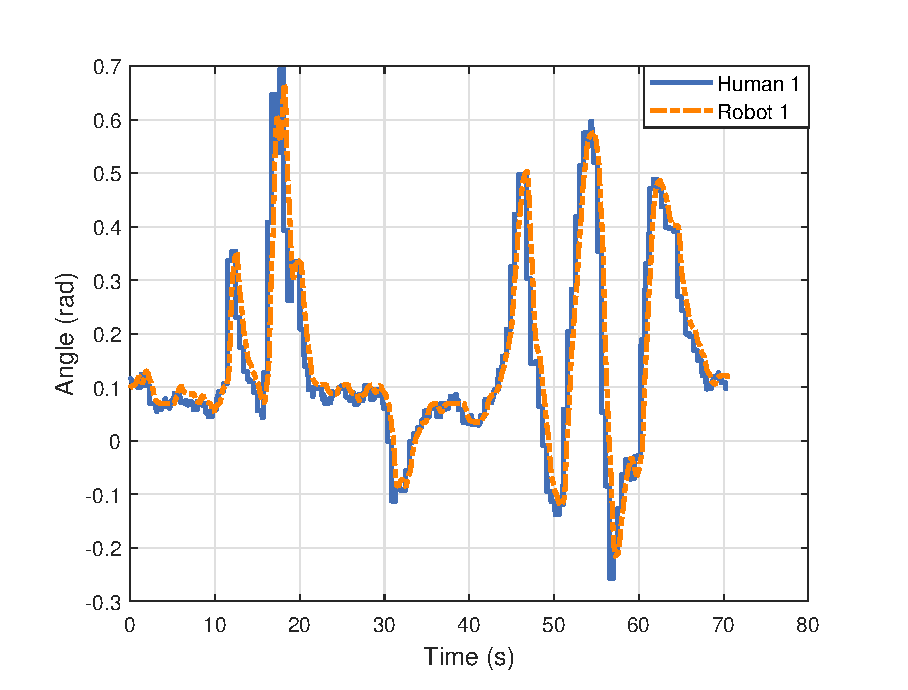
\includegraphics[width=7cm]{Figure/chapter2/Fig13a.eps}}
		 \hfill  % 调整两图之间的间距
		\subfloat[\centering]{\includegraphics[width=7cm]{Figure/chapter2/Fig13b.eps}}\\
		\subfloat[\centering]{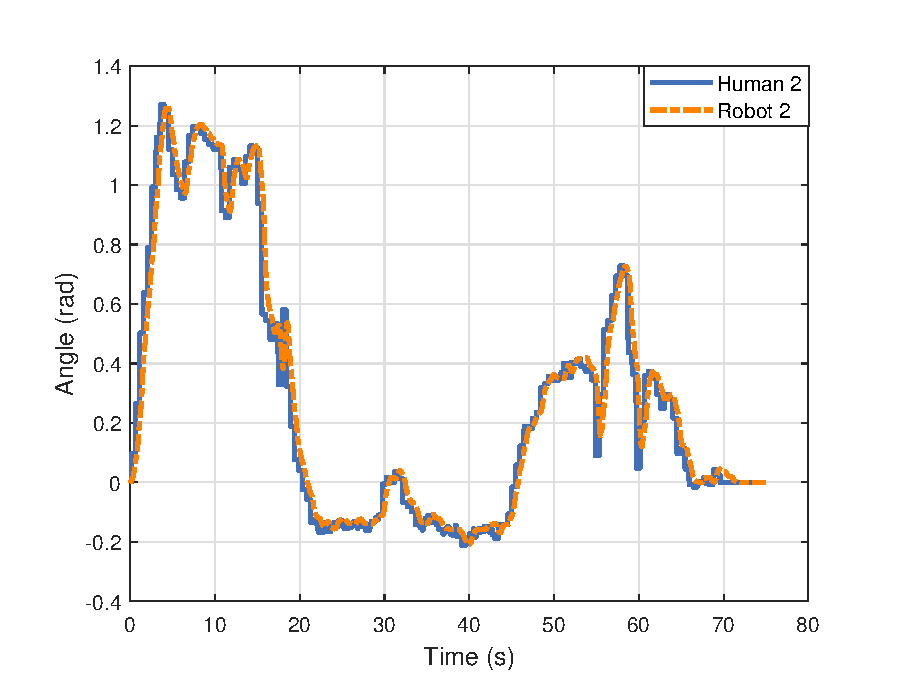
\includegraphics[width=7cm]{Figure/chapter2/Fig13c.eps}}
		\hfill  % 调整两图之间的间距
		\subfloat[\centering]{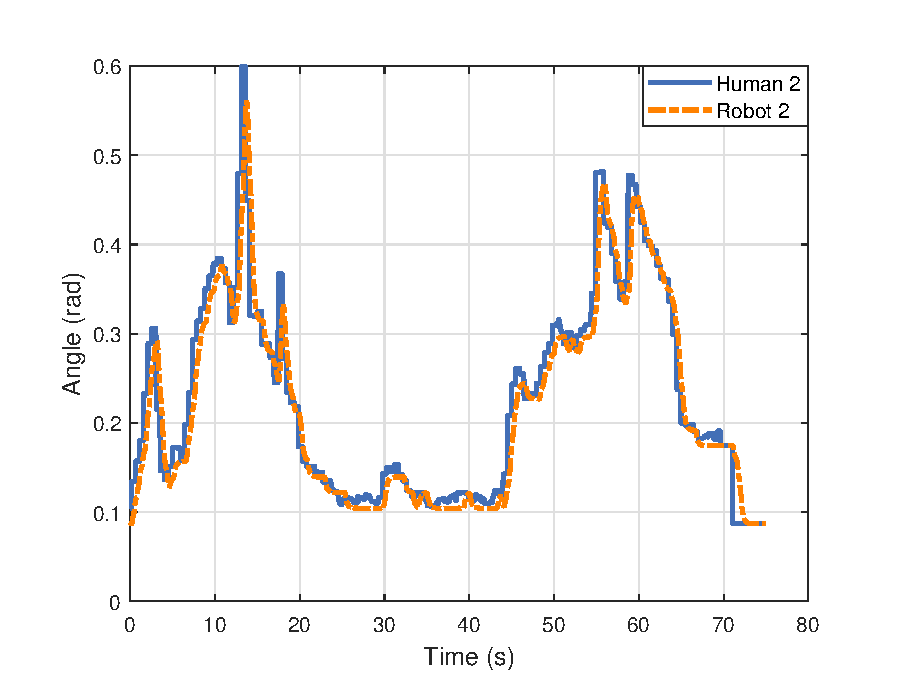
\includegraphics[width=7cm]{Figure/chapter2/Fig13d.eps}}
		
	\end{adjustwidth}
\caption{双人动作模仿中左肩屈伸关节和外展-内收关节的轨迹跟踪:(\textbf{a})和(\textbf{b})机器人 1 跟踪表演者 1 左肩屈伸关节和外展-内收关节的关节轨迹;(\textbf{c})和(\textbf{d})机器人 2 跟踪表演者 2 左肩屈伸关节和外展-内收关节的关节轨迹。}

\label{fig:Tracking of Robot Arm Joints dual}
\end{figure} 

\begin{figure}[H]
	\centering
	\begin{adjustwidth}{0cm}{0cm}
		\subfloat[\centering]{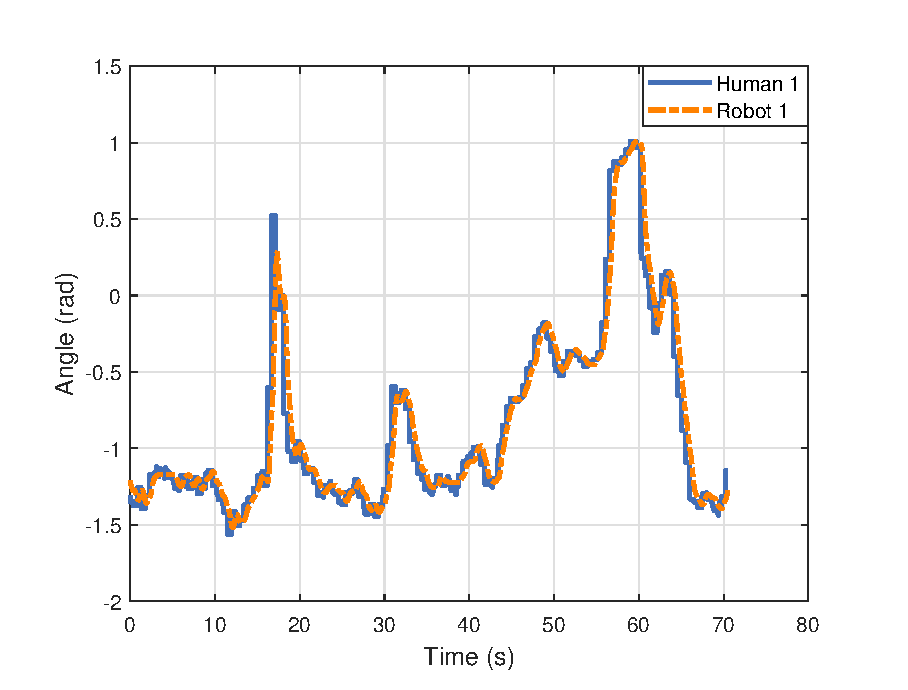
\includegraphics[width=7cm]{Figure/chapter2/LSY1.eps}}
		\hfill  % 调整两图之间的间距
		\subfloat[\centering]{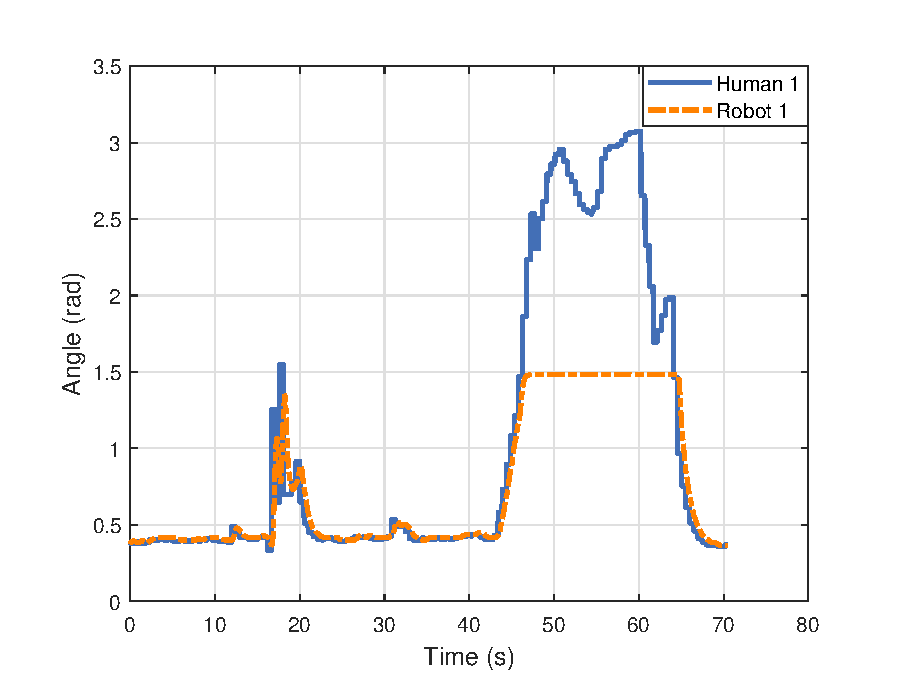
\includegraphics[width=7cm]{Figure/chapter2/LE1.eps}}\\
		\subfloat[\centering]{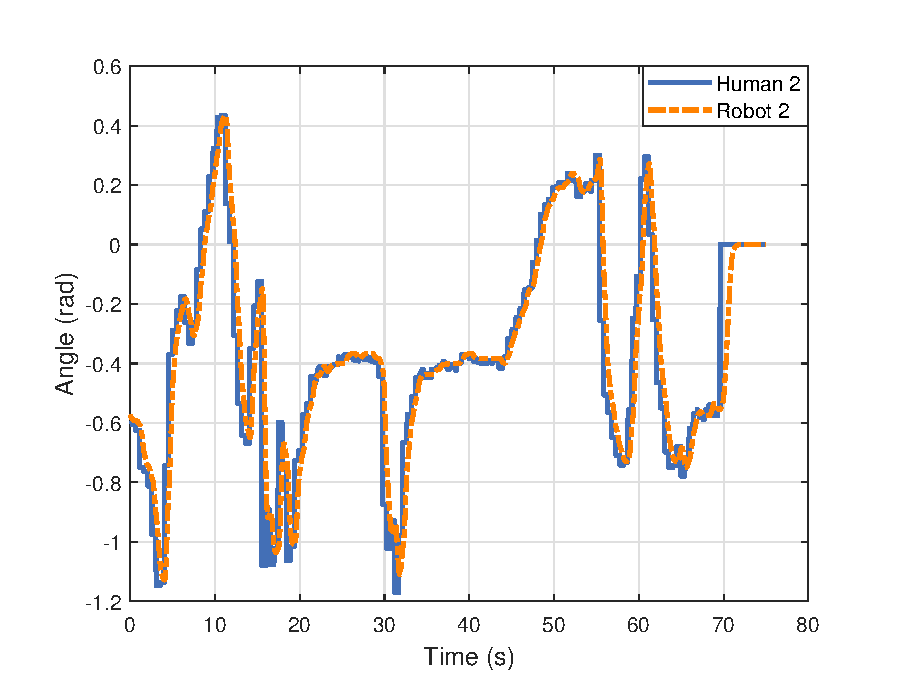
\includegraphics[width=7cm]{Figure/chapter2/LSY2.eps}}
		\hfill  % 调整两图之间的间距
		\subfloat[\centering]{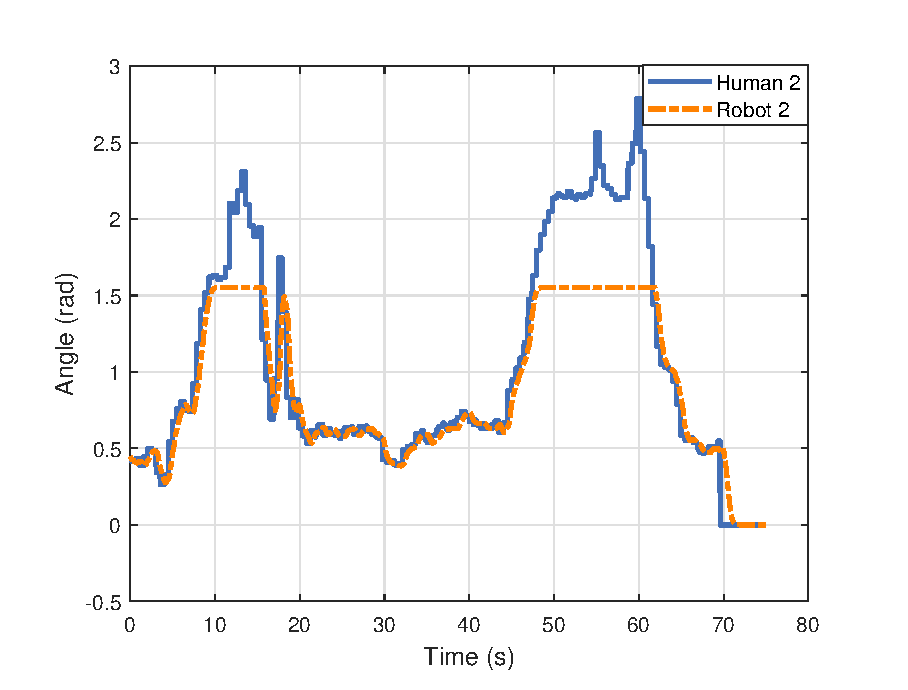
\includegraphics[width=7cm]{Figure/chapter2/LE2.eps}}
		
	\end{adjustwidth}
	\caption{双人动作模仿中左肩关节外旋-内旋及肘关节的轨迹跟踪:(\textbf{a})和(\textbf{b})表示机器人 1 跟踪示范者 1 左肩关节外旋-内旋及肘关节的轨迹;(\textbf{c})和(\textbf{d})表示机器人 2 跟踪示范者 2 左肩关节外旋-内旋及肘关节的轨迹。
}
	\label{fig:Robot Arm Joints dual}
\end{figure} 

为了定量评估动作模仿的跟踪性能,本文采用均方误差(Mean Square Error, MSE)作为关节轨迹跟踪精度的指标。MSE 值越小,表示机器人的关节运动越接近目标轨迹。

图 \ref{fig:MSE} 展示了单人和双人动作模仿过程中各关节的均方误差(MSE)。由于关节电机存在固有延迟,跟踪过程中不可避免地引入了误差,从而影响了 MSE 值。结果表明,与单人动作模仿相比,双人动作模仿时各关节的 MSE 并未显著增加,这验证了系统在多智能体动作模仿中的可行性和有效性。此外,肩部外展-内收关节的跟踪 MSE 最小,而肩部内外旋关节的跟踪 MSE 最大。这主要是因为肩部外展-内收的运动特征更为显著,使得从姿态估计输出的人体关键点数据更稳定。因此,通过几何建模计算得到的肩部外展-内收关节参考角波动较小。相比之下,手腕深度信息的波动较大,使得生成的关键点数据变化更明显,导致肩部内外旋关节参考角的波动较大。总之,关节跟踪 MSE 主要来源于姿态估计过程中的数据波动,同时电机响应延迟也会对跟踪精度产生一定影响。
\begin{figure}[H]
	\centering
	\begin{adjustwidth}{0cm}{0cm}
		\subfloat[\centering]{\includegraphics[width=7cm]{Figure/chapter2/Fig14_a.eps}}
		\label{fig:MSE_1}
	    \hfill  % 调整两图之间的间距
		\subfloat[\centering]{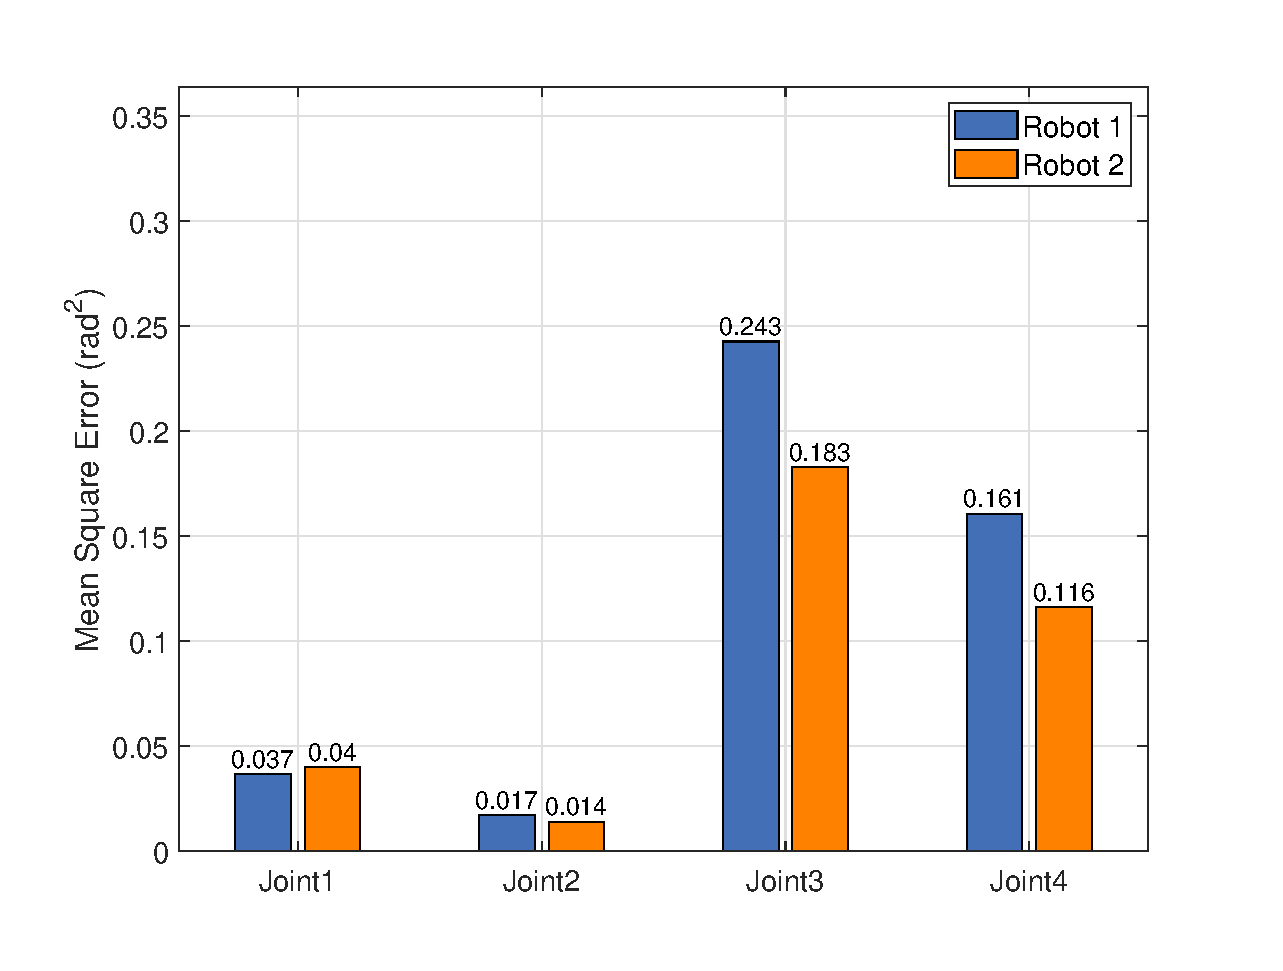
\includegraphics[width=7cm]{Figure/chapter2/Fig14_b.eps}}
		\label{fig:MSE_2}
		
	\end{adjustwidth}
\caption{手臂动作模仿过程中关节角度的均方误差(MSE):(\textbf{a})单人手臂动作模仿;(\textbf{b})双人手臂动作模仿。关节 1 对应肩屈伸关节,关节 2 对应肩外展-内收关节,关节 3 对应肩外旋-内旋关节,关节 4 对应肘屈伸关节。}

\label{fig:MSE}
\end{figure} 

\subsection{消融实验}
通过消融实验,我们比较了仅使用几何方法以及基于优化的二次规划(QP)方法在末端执行器位置跟踪任务中的性能。如表~\ref{tab1} 所示,当采用纯几何方法时,末端执行器的跟踪误差为 $9.35 \times 10^{-2}$;而采用 QP 优化方法时,该误差显著降低至 $3.75 \times 10^{-4}$。相比之下,本文提出的方法将末端执行器的跟踪误差进一步降低至 $2.065 \times 10^{-5}$,略高于解析逆向运动学方法,但明显优于几何方法和 QP 方法。


在机器人任务执行中,末端执行器的跟踪精度固然重要,但保持合理的手臂构型同样关键。良好的手臂构型不仅可以避免与环境及机器人自身发生碰撞,还能增强运动的稳定性与安全性。如表 \ref{tab1} 所示,只有本文提出的改进重定向方法在保持可行手臂构型的同时,实现了较小的末端执行器误差。
\begin{table}[ht]
	\centering
	\caption{不同重定向方法的性能比较}
	\begin{tabular}{lcccc}
		\toprule
		方法       & 关节限制 & 构型约束 & 末端执行器误差  & 迭代次数 \\
		\midrule
		几何方法     & $\times$     & \checkmark    & \(9.35 \times 10^{-2}\)    & $\times$   \\
		解析逆运动学 & $\times$     & $\times$      & \(2\times 10^{-6}\)     & 1          \\
		QP方法       & \checkmark   & $\times$      &  \(3.75\times 10^{-4}\) & $\approx100 $      \\
		改进重定向     & \checkmark   & \checkmark    &  \(2.065\times 10^{-5}\)  & $\approx20 $       \\
		\bottomrule
	\end{tabular}
	\label{tab1}
\end{table}

此外,在计算效率方面,所提出的方法仅需约 20 次迭代即可收敛至最优解,相较于传统的基于 QP 的方法,更适合实时应用。

为了直观比较不同重定向方法在动作模仿任务中的表现,我们提供了本文所提出方法的实验视频(\href{https://youtu.be/lXEJFHylUEI}{实验视频}),并在同一关键帧下展示了各重定向方法的差异。如图~\ref{fig:matched_com} 所示,实验结果表明:


基于几何的方法通过追踪肩关节和肘关节角度来保证手臂的配置相似性。然而,由于它并未显式地追踪末端执行器的位置,因此末端执行器的跟踪误差相对较大。逆向运动学(IK)方法能够实现末端执行器位置的跟踪,但由于在求解过程中未考虑关节限制且忽略手臂配置,导致肘关节位置偏差明显,手臂配置相似性降低。QP 方法在优化关节限制的同时能够成功跟踪末端执行器位置,并改善手臂配置。然而,该方法增加了计算复杂度,且手臂配置仍存在一定误差。我们提出的改进重定向方法在保持低末端执行器跟踪误差的同时,能够维持手臂的相似配置,从而提升运动的稳定性和自然性。

为了评估多机器人动作模仿的自然性和可接受性,我们邀请了六名参与者进行示范动作,随后机器人执行模仿及任务操作。评价指标如下:
1. **动作平滑性 (Motion Smoothness, MS)**:评估机器人执行过程中是否存在不连续或突兀的动作。
2. **姿态可行性 (Pose Feasibility, PF)**:评估机器人手臂姿态是否与人类示范者保持相似。
3. **任务完成度 (Task Achievement, TA)**:评估机器人是否准确完成指定的模仿任务。
4. **总体用户偏好 (Overall User Preference)**:反映参与者对整体模仿质量的主观评价。

 用户评分采用1(差)到5(优)的五分制,统计结果如表 \ref{tab2} 所示。实验结果表明,在所有评价指标上,我们的方法均优于基于几何方法(geometry-based)、逆向运动学(IK)和二次规划(QP)方法。尤其在动作平滑性和姿态可行性方面,用户主观评分明显更高。这表明,改进的重定向方法不仅提高了模仿精度,同时也增强了动作的自然性和用户可接受性。

 \subsection{局限}
 所提出的改进重定向算法能够有效地计算出最优关节角,同时满足手臂几何结构一致性和末端执行器位置跟踪的要求。通过结合多人人体姿态估计技术,该框架实现了多机械臂的动作模仿与协作任务,增强了系统的适应性和多任务处理能力。尽管人体运动运动学长期以来一直是研究前沿,但本研究在重定向算法方面相较于现有方法取得了进展。尤其是,将改进的重定向算法与多机器人协作任务相结合,并利用实时人体姿态估计进行机器人动作模仿,本方法在复杂环境中显著提升了动作模仿的精度与协调性。
 然而,所提出的框架仍存在一定局限性,尤其是在姿态方向跟踪方面。由于我们的姿态估计系统主要通过单目相机估计末端执行器的位置,它只能获取位置数据,而无法完整提取关节的全姿态信息(包括旋转分量)。这一限制显著影响了关节运动的灵活性,尤其是在涉及前臂旋前-旋后和手腕屈伸等复杂动作时,机器人无法充分调整这些关节以满足任务要求。未来的研究可以引入完整的姿态估计,实现位置与方向的综合跟踪,从而提升机器人在复杂任务中的灵活性与精度。关于关节限位约束,如图 \ref{fig:Robot Arm Joints dual} (b) 和 (d) 所示,无法实现精确跟踪主要是由于机械结构限制了关节运动范围,这一问题在传统控制方法中同样存在。为解决该局限性,未来工作可引入更加灵活的自适应关节限位控制策略,使机器人在不超出机械极限的前提下调整运动范围,从而减轻关节限位带来的影响。

\begin{figure}[h]
	\centering
	\begin{minipage}{0.48\linewidth}
		\centering
		\captionof{table}{不同重定向方法的用户主观评价}
		\begin{tabular}{lcccc}
			\toprule
			方法  & MS  & PF  & TA  & 综合评分 \\
			\midrule
			几何方法     & 4   & 5   & 2   & 4   \\ 
			逆运动学方法 & 4   & 2   & 3   & 2   \\
			QP 方法      & 3   & 3   & 3   & 3   \\
			本文方法     & 5   & 5   & 4   & 5   \\
			\bottomrule
		\end{tabular}
		\label{tab:user_evaluation}
	\end{minipage}
	\hfill
	\begin{minipage}{0.5\linewidth}
		\centering
		\includegraphics[width=\linewidth]{Figure/chapter2/mathed_com.png}
		\caption{相同动作关键帧下不同重定向方法的对比结果。橙色点表示目标位置,蓝色点表示实际到达位置。}
		\label{fig:matched_comparison}
	\end{minipage}
\end{figure}

\section{结论}
本文提出了一个综合性的实时多仿人机器人手臂动作模仿框架,该框架采用改进的重定向方法,有效实现了手臂运动学配置与末端执行器精度之间的最佳平衡。通过整合多人人体姿态估计技术,该框架不仅支持多仿人机器人之间的协作运动,还为复杂任务中的多机器人协作提供了有效解决方案。

实验结果表明,机器人能够成功复现各种人类手臂动作。尽管随着示范者数量的增加,姿态估计误差有所上升,但整体动作模仿仍保持较高的跟踪精度和末端执行器准确性。此外,在倒水、物品分类及协作等任务中,我们进一步验证了改进重定向方法在保持手臂运动学结构完整性和末端执行器精度方面的优越性能。此外,随着多人人体姿态估计技术的整合,即使检测对象数量增加,系统仍能保持良好的实时性能,有效避免了计算负载的大幅增加。

尽管该框架在高精度与高效率方面表现出色,但在姿态跟踪上仍存在一定局限性。未来的研究将重点进一步优化姿态估计技术,实现位置与姿态的综合跟踪,从而提升机器人在复杂任务中的灵活性与精度,并使其在多智能体交互与协作任务中发挥更大作用。